\chapter{Experimental}
\label{experimental}
This chapter will show the complete developement process of the Electronic Leadscrew based on the V-Modell. 


\section{Requirements and Logical Architecture}

In this section the developement process in the first part of the V-Modell will be described. As shown in figure \ref{V Model Requirements} this part is split into two. The requirements describe the fundamental properties of the system in order to function.
The system Logical Architecture describes how the different system components are supposed to interact with each other.

\begin{figure}[h!]
    \begin{center}
    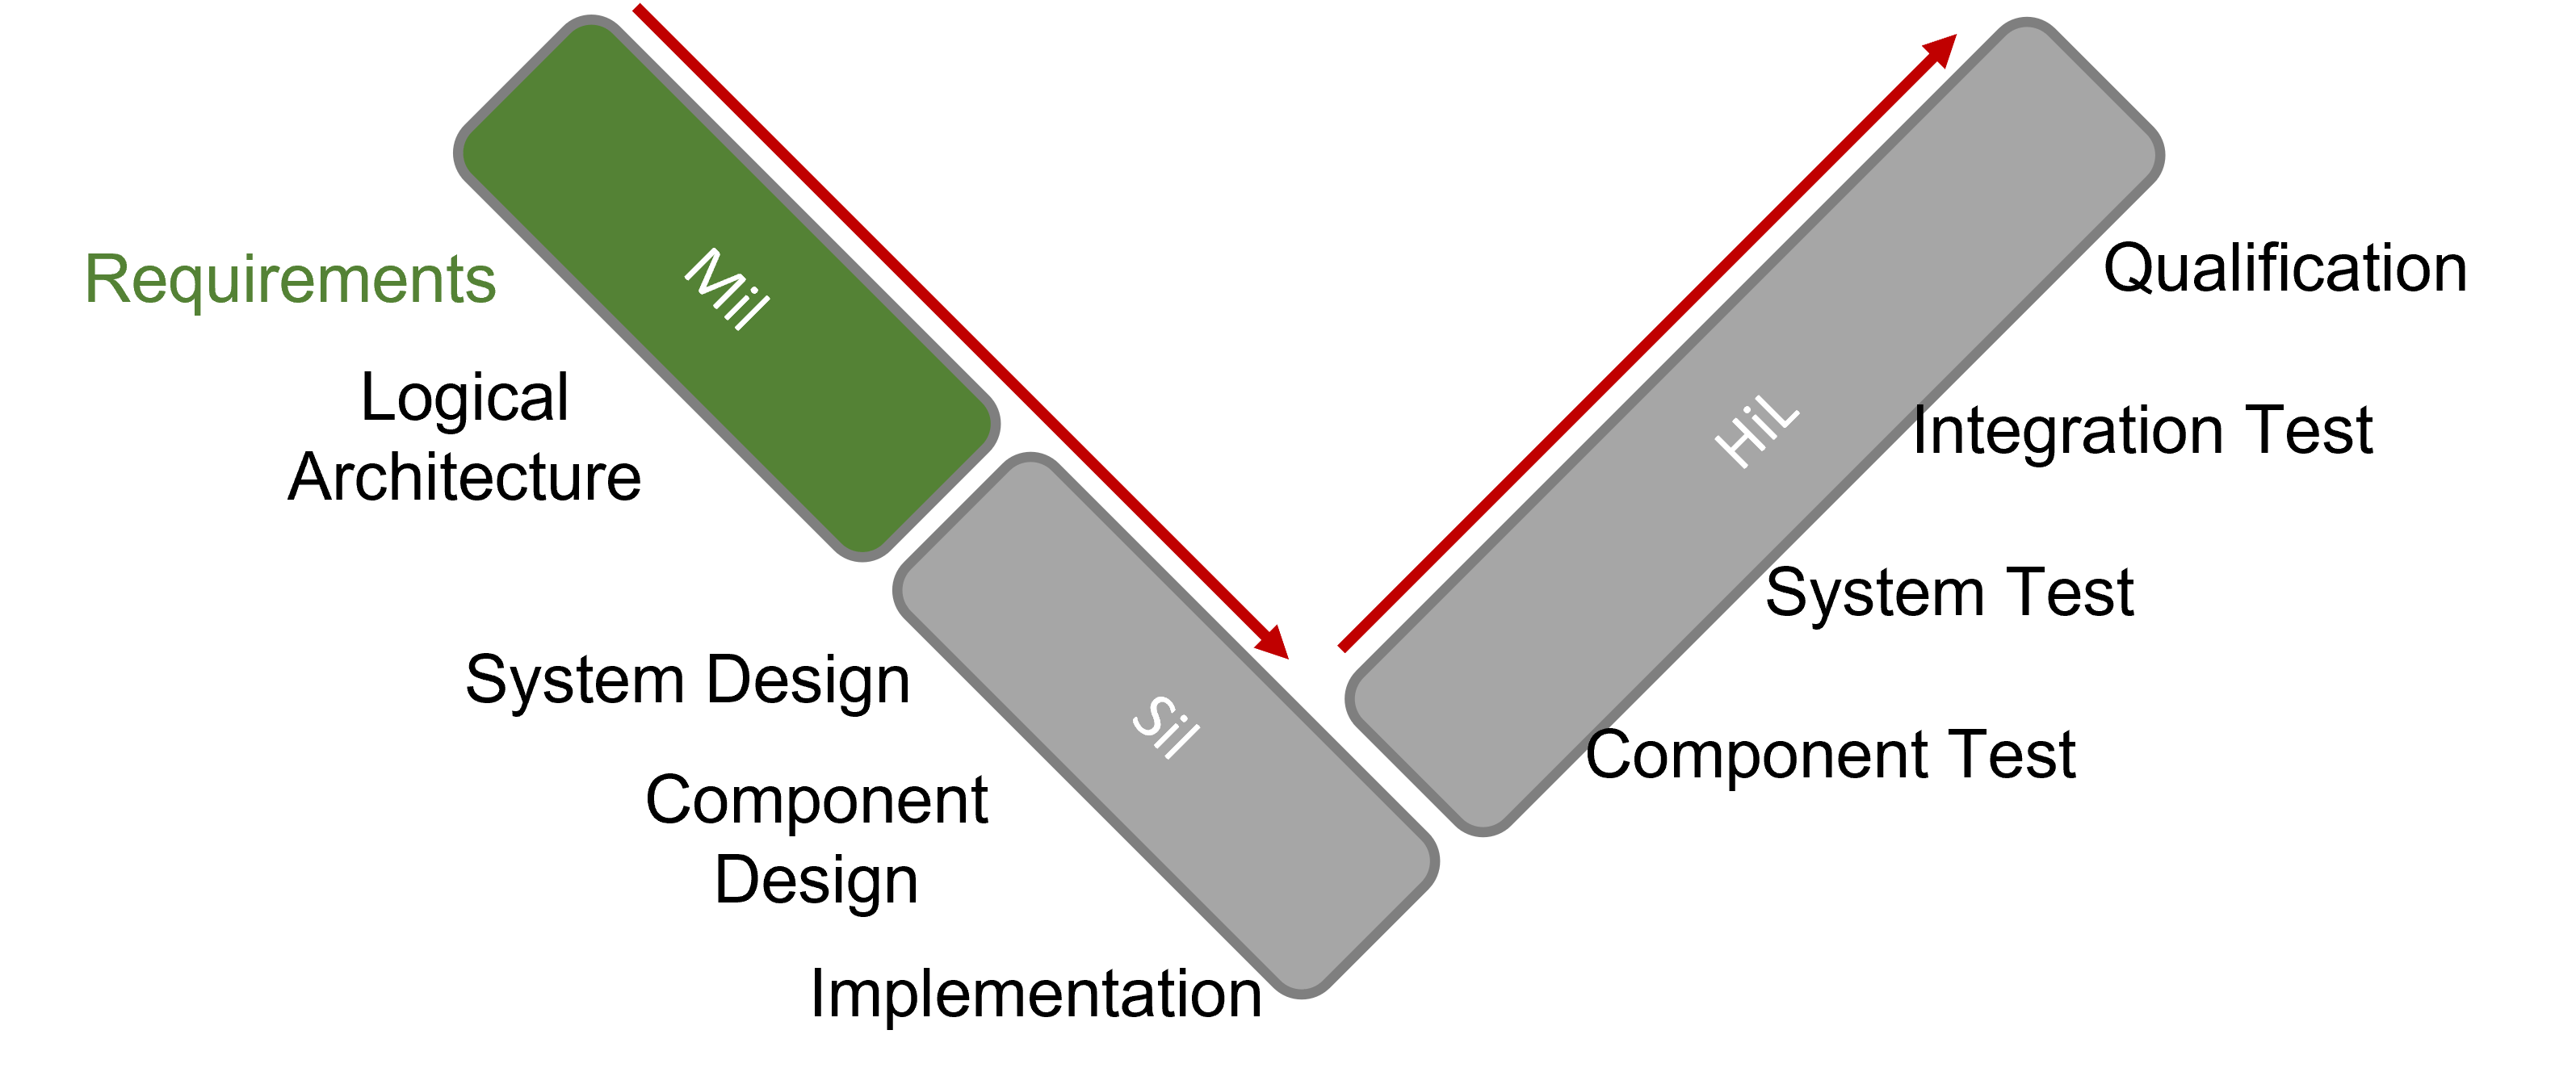
\includegraphics[width=12cm]{Pictures/V Model Requirements.png}
    \caption[V Model Requirements]{V Model Requirements Stage; Green - Developement status}
    \label{V Model Requirements}
    \end{center}
\end{figure}


\subsection{Requirements}
The developement of the System requirements was the first step in the developement process. This first step is one of the most important steps in the developement process, because it defines the functions and properties of all Systemcomponents.A selectoin of the requirements for the Human Machine Interface (HMI), the micro controller ($\mu$C), the motor and the motor controller are shown in Table \ref{Tab Key Requirements}. The full list of requirements can be found in Appendix \ref{AppendixRequirements}.

\begin{table}
    \centering
     \begin{tabular}{||c|c|c|c|c||} 
        \hline
        Req. Nr. & HMI & $\mu$C & Motor & Motor Controller \\ [0.5ex] 
        \hline\hline
        1 & Touch       & Real Time         &  Max. Torqe   & Closed Loop   \\ 
        2 & Modular     & Matlab Code Gen.  &  Min. Torqe   & Supply Voltage\\
        3 & UART Com.   & UART Com.         &  Max. Speed   & Programmable  \\
        4 & Separat PS  & Quad. Encoder     &  Min. Speed   & Resolution    \\
        5 & Mount       & GPIO              &  Space Claim  & Communication \\ [1ex] 
        \hline
     \end{tabular}
     \caption{Selection of Key Requirements for the ELS}
     \label{Tab Key Requirements}
\end{table}




\subsection{Logical Architecture}

The next step in the developement process of the ELS was to create the Logical Architecture of the System. This was done as a Toplevel Blockdiagramm as shown in Figure \ref{Logical Architecture}.

\begin{figure}[h!]
    \begin{center}
    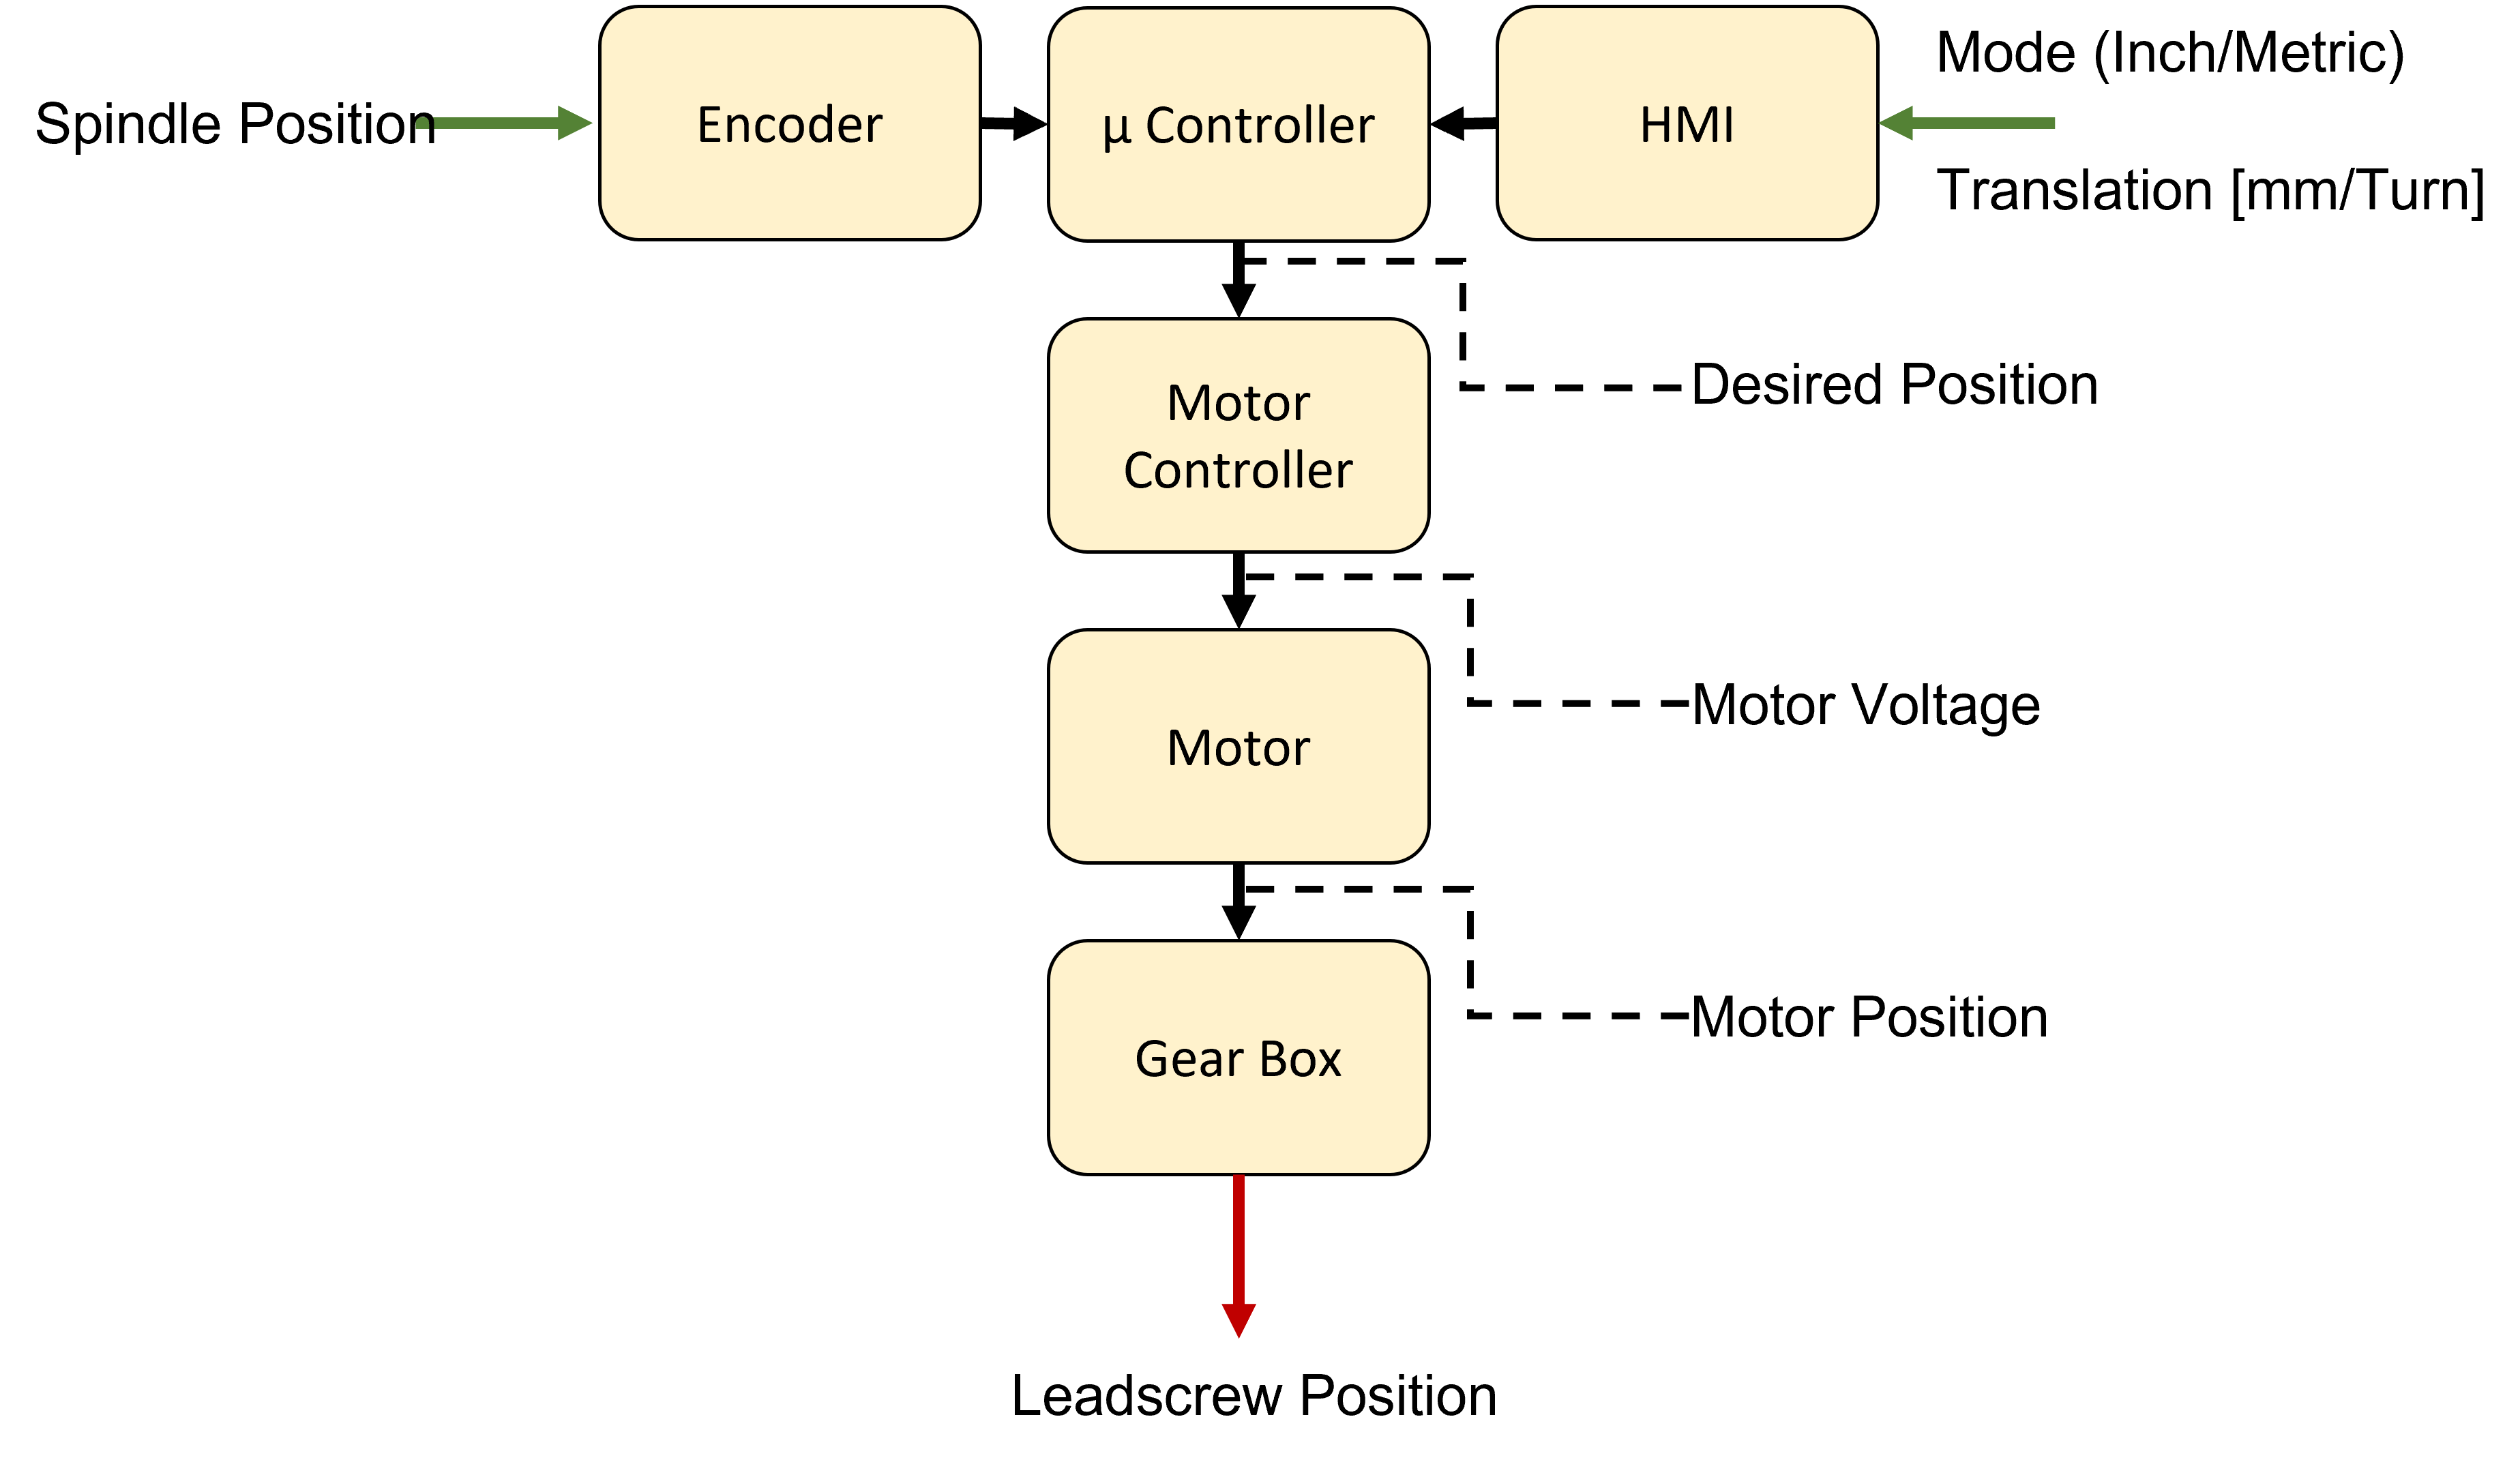
\includegraphics[width=12cm]{Pictures/Logical Architecture.png}
    \caption[Logical Architecture]{Logical Architecture}
    \label{Logical Architecture}
    \end{center}
\end{figure}

\section{System Design and Implementation}
This section describes the second half of the developement process, divided into system and component design as well as the integration of the components. This is the most time consuming process of the developement.For the system and component design, every function of each system and subsystem must be specified in detail. During the implementation phase, these functions are than transferred into the real system.\\
This developement stage is represented by the Software in the Loop (SIL) stage and is shown in Figure \ref{V Model System Design}.

\begin{figure}[h!]
    \begin{center}
    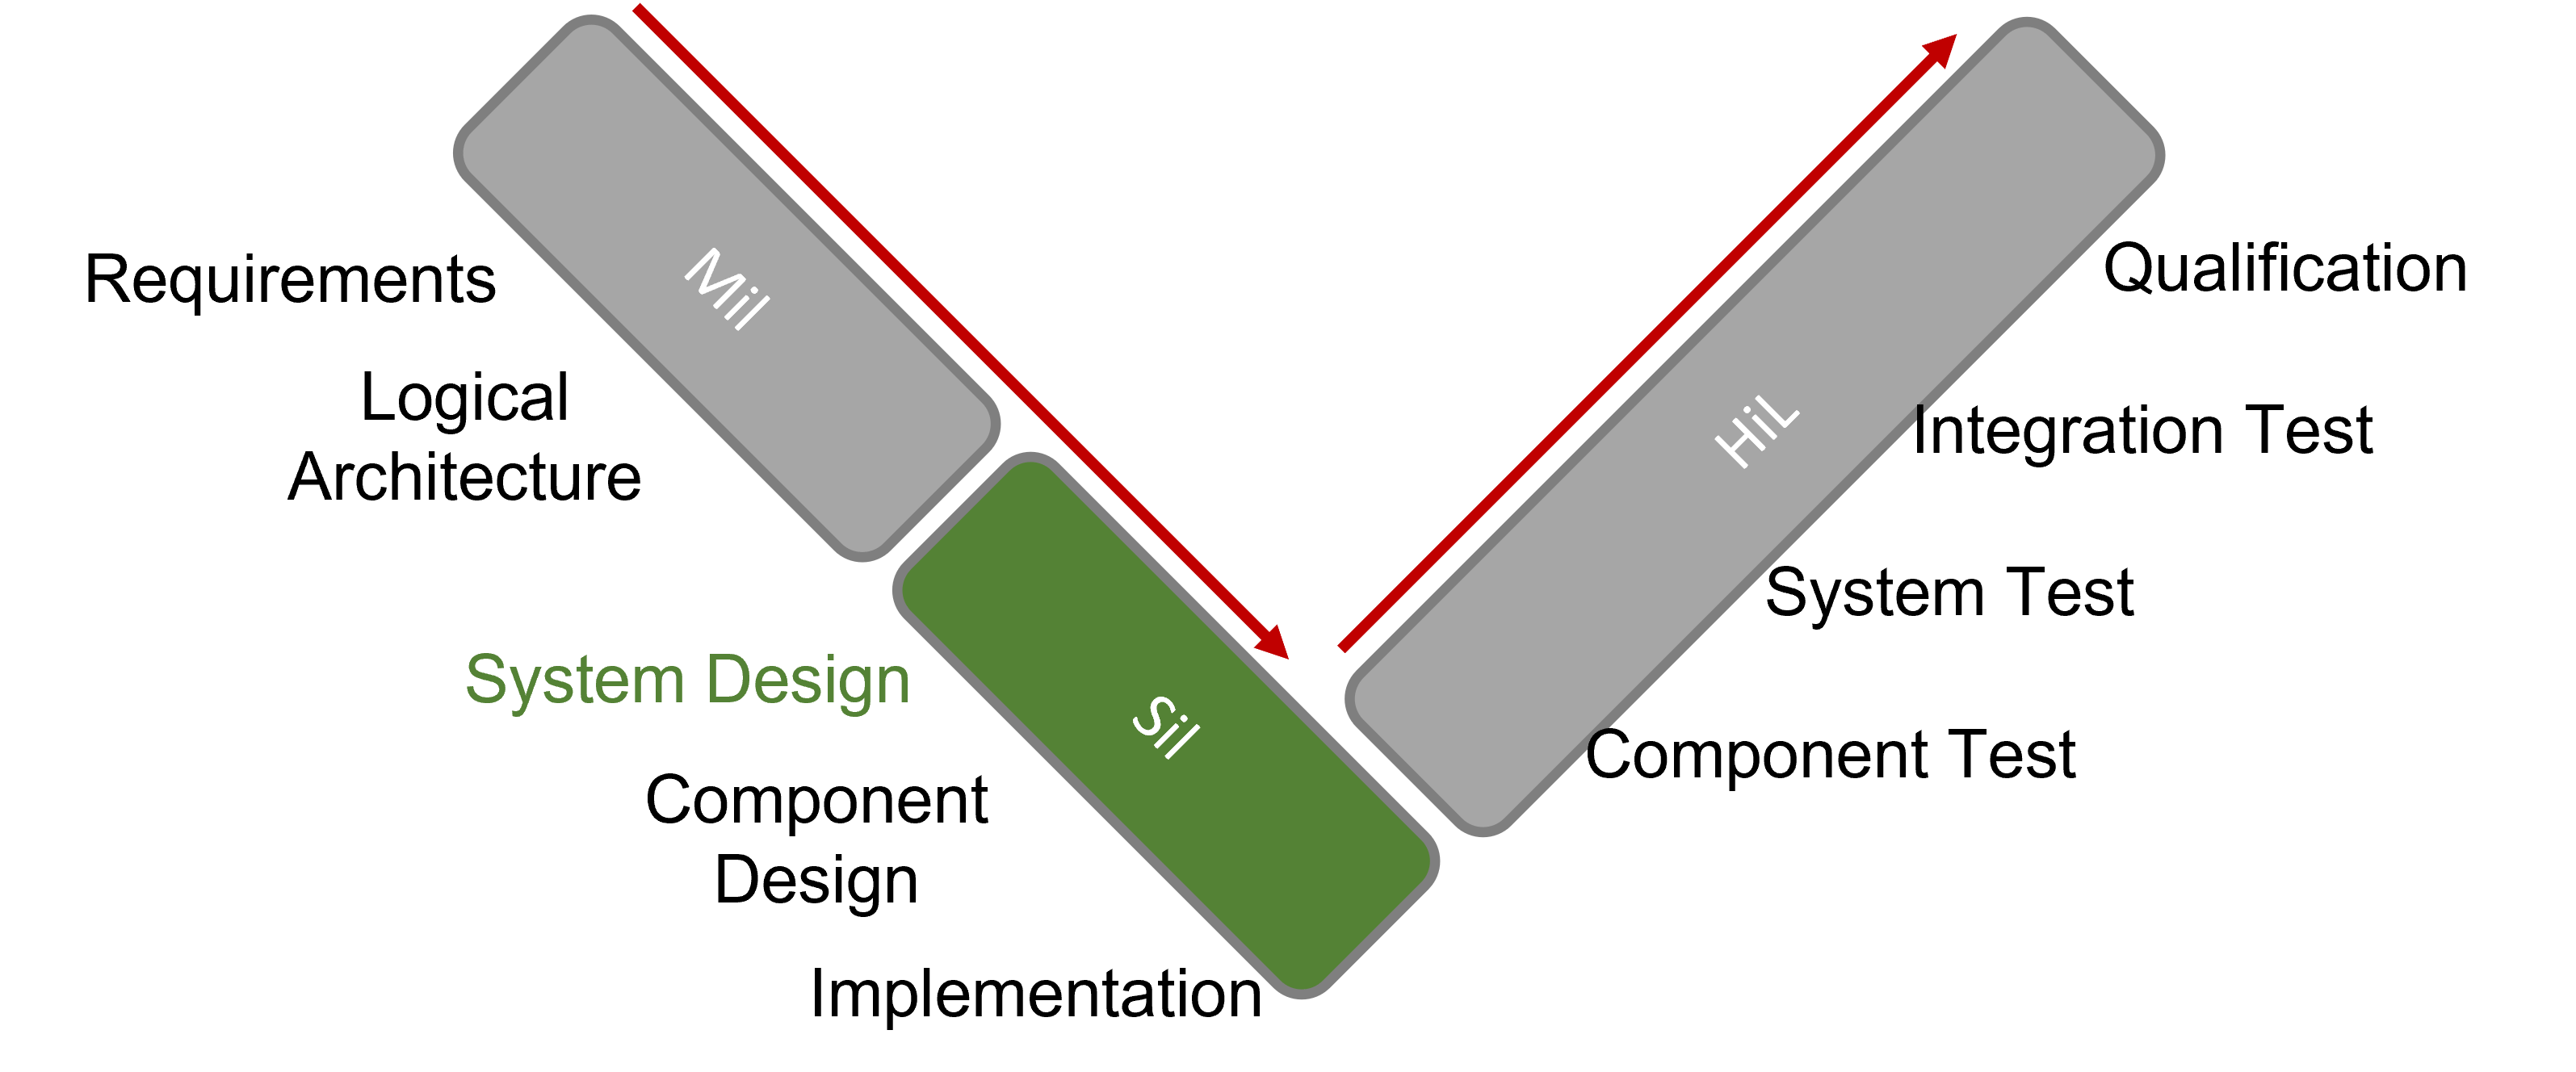
\includegraphics[width=12cm]{Pictures/V Model System Design.png}
    \caption[V Model System Design]{V Model SIL Stage; green - Developement steps SIL stage}
    \label{V Model System Design}
    \end{center}
\end{figure}

\subsection{System Design}

\subsection{Component Design}
\subsubsection{HMI}
\subsubsection{Micro Controller}
\subsubsection{Encoder}
%%TODO Put Opkon in Appendix List of Companies
The design or in this case selection of the encoder was purely based on the previously defined requirements. The most significant requirements are shown in Table \ref{Tab Encoder Key Requirements}.

\begin{table}
    \centering
     \begin{tabular}{||c|c|c||} 
        \hline
        Req. Nr. & Requirement & Value\\ [0.5ex] 
        \hline\hline
        1 & Physical Size       & 60mm		\\ 
        2 & Supply Voltage      & 5V        \\
        3 & Resolution          & 4096 ppt  \\
        4 & Directional         & Yes       \\[1ex] 
        \hline
     \end{tabular}
     \caption{Selection of Key Requirements for the ELS}
     \label{Tab Encoder Key Requirements}
\end{table}

This lead to the selection of a Encoder from the manufacturer Opkon (see Appendix \ref{AppendixListOfCompanies}). The Encoder creates 4096 pulses/revolution, with half of them phase shifted by 90\degree in order to determine the turning direction. Further, the encoder covers an input voltage range from 5V - 30V, which is compatible with the Encoder Pins on the Launchpad XL. With a hight of 57mm, the Encoder just fits into the previously determined specifications.

\subsubsection{Motor and Motor Controller}
%%TODO Put Steppers Online in Appendix List of Companies
The motor was selected based the requirements list as well as recommendations from James Clough \cite{CloughELS}. The selected motor is from the company Steppers Online (see Appendix \ref{AppendixListOfCompanies}). It is a so called "integrated servo moter". This means, the motor consist of a brushless DC-motor, an encoder as well as the corresponding motor controller. All three of these parts are packaged into one unit as shown in Figure \ref{Integrated Servo Motor}.\\

\begin{figure}[h!]
    \begin{center}
    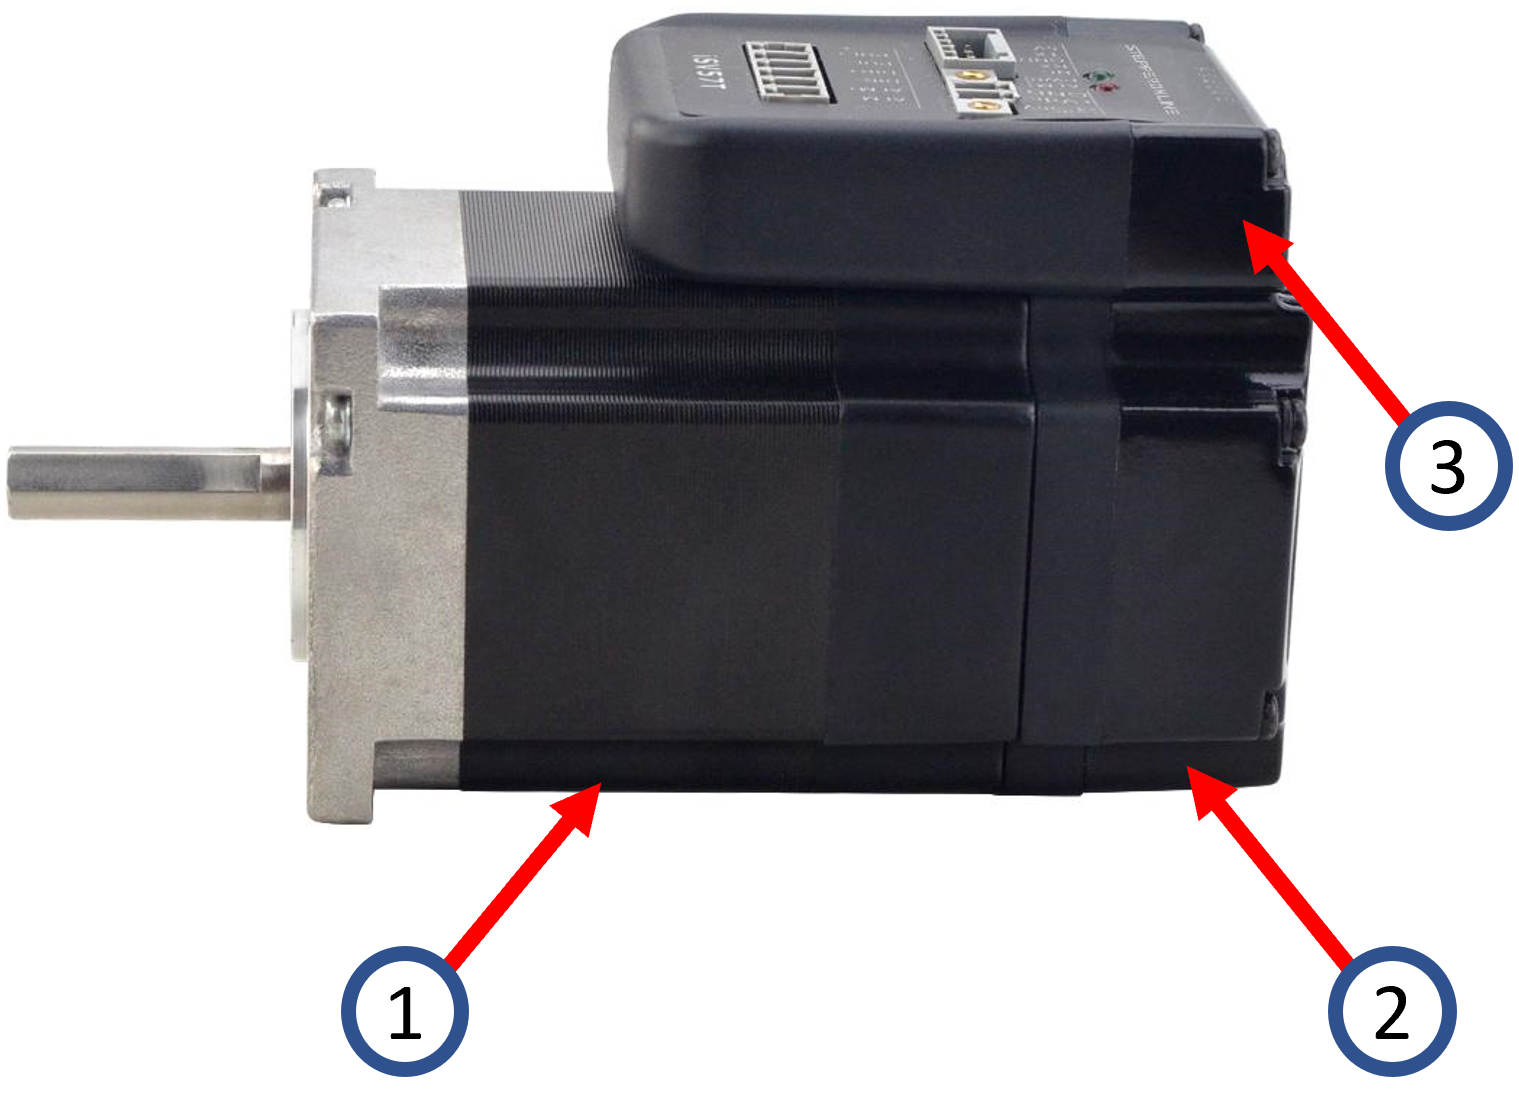
\includegraphics[width=12cm]{Pictures/IntegratedServo.png}
    \caption[Integrated Servo Motor]{Integrated Servo Motor; 1 - BLDC Motor, 2 - Encoder Unit, 3 - Control Unit}
    \label{Integrated Servo Motor}
    \end{center}
\end{figure}

The motor features an RPM range from 0 to 4000 rpm and a very constant maximum torque of 0.4 nm. Further, it has the right dimensions in order to fit the space claim requirements.\\
The motor controller in combination with the required software represent an easy programming interface. Via this interface, control parameters as well as parameter for the dynamics and precision of the motor can be set. As a starting value, the motor stiffness (responsiveness) gain was set to its maximum. Based on the software design of the micro controller, the precision of the motor was set to 2000 steps/revolution.\\
The interface to the motor is provided by a simple digital protocol. It consists of a direction and a step pin. The direction reacts to a logical 5V signal, where a logical 1 (5V) corresponds to clockwise rotation and a logical 0 (0V) corresponds to counterclockwise rotation. The step input reacts to logical pulses with a minimum pulse width of 1$\mu$s. Each puls will than move the motor by $\frac{1}{motor-resulution}$.

\subsubsection{Gearbox}
Because the motor is mounted underneath the leadscrew, a a coupling between both elements was needed. This was done with the already existing gears from the old gearbox of the lathe. This decision was made because it needed the least modification (only a coupler from the motor to the gear had to be manufactured) and was the cheapest option. The gear ratio of 25/80 was selected to optimze the feed range of the lathe with the available RPM of the motor. This is shown in Figure

\section{System Testing}
\begin{figure}[h!]
    \begin{center}
    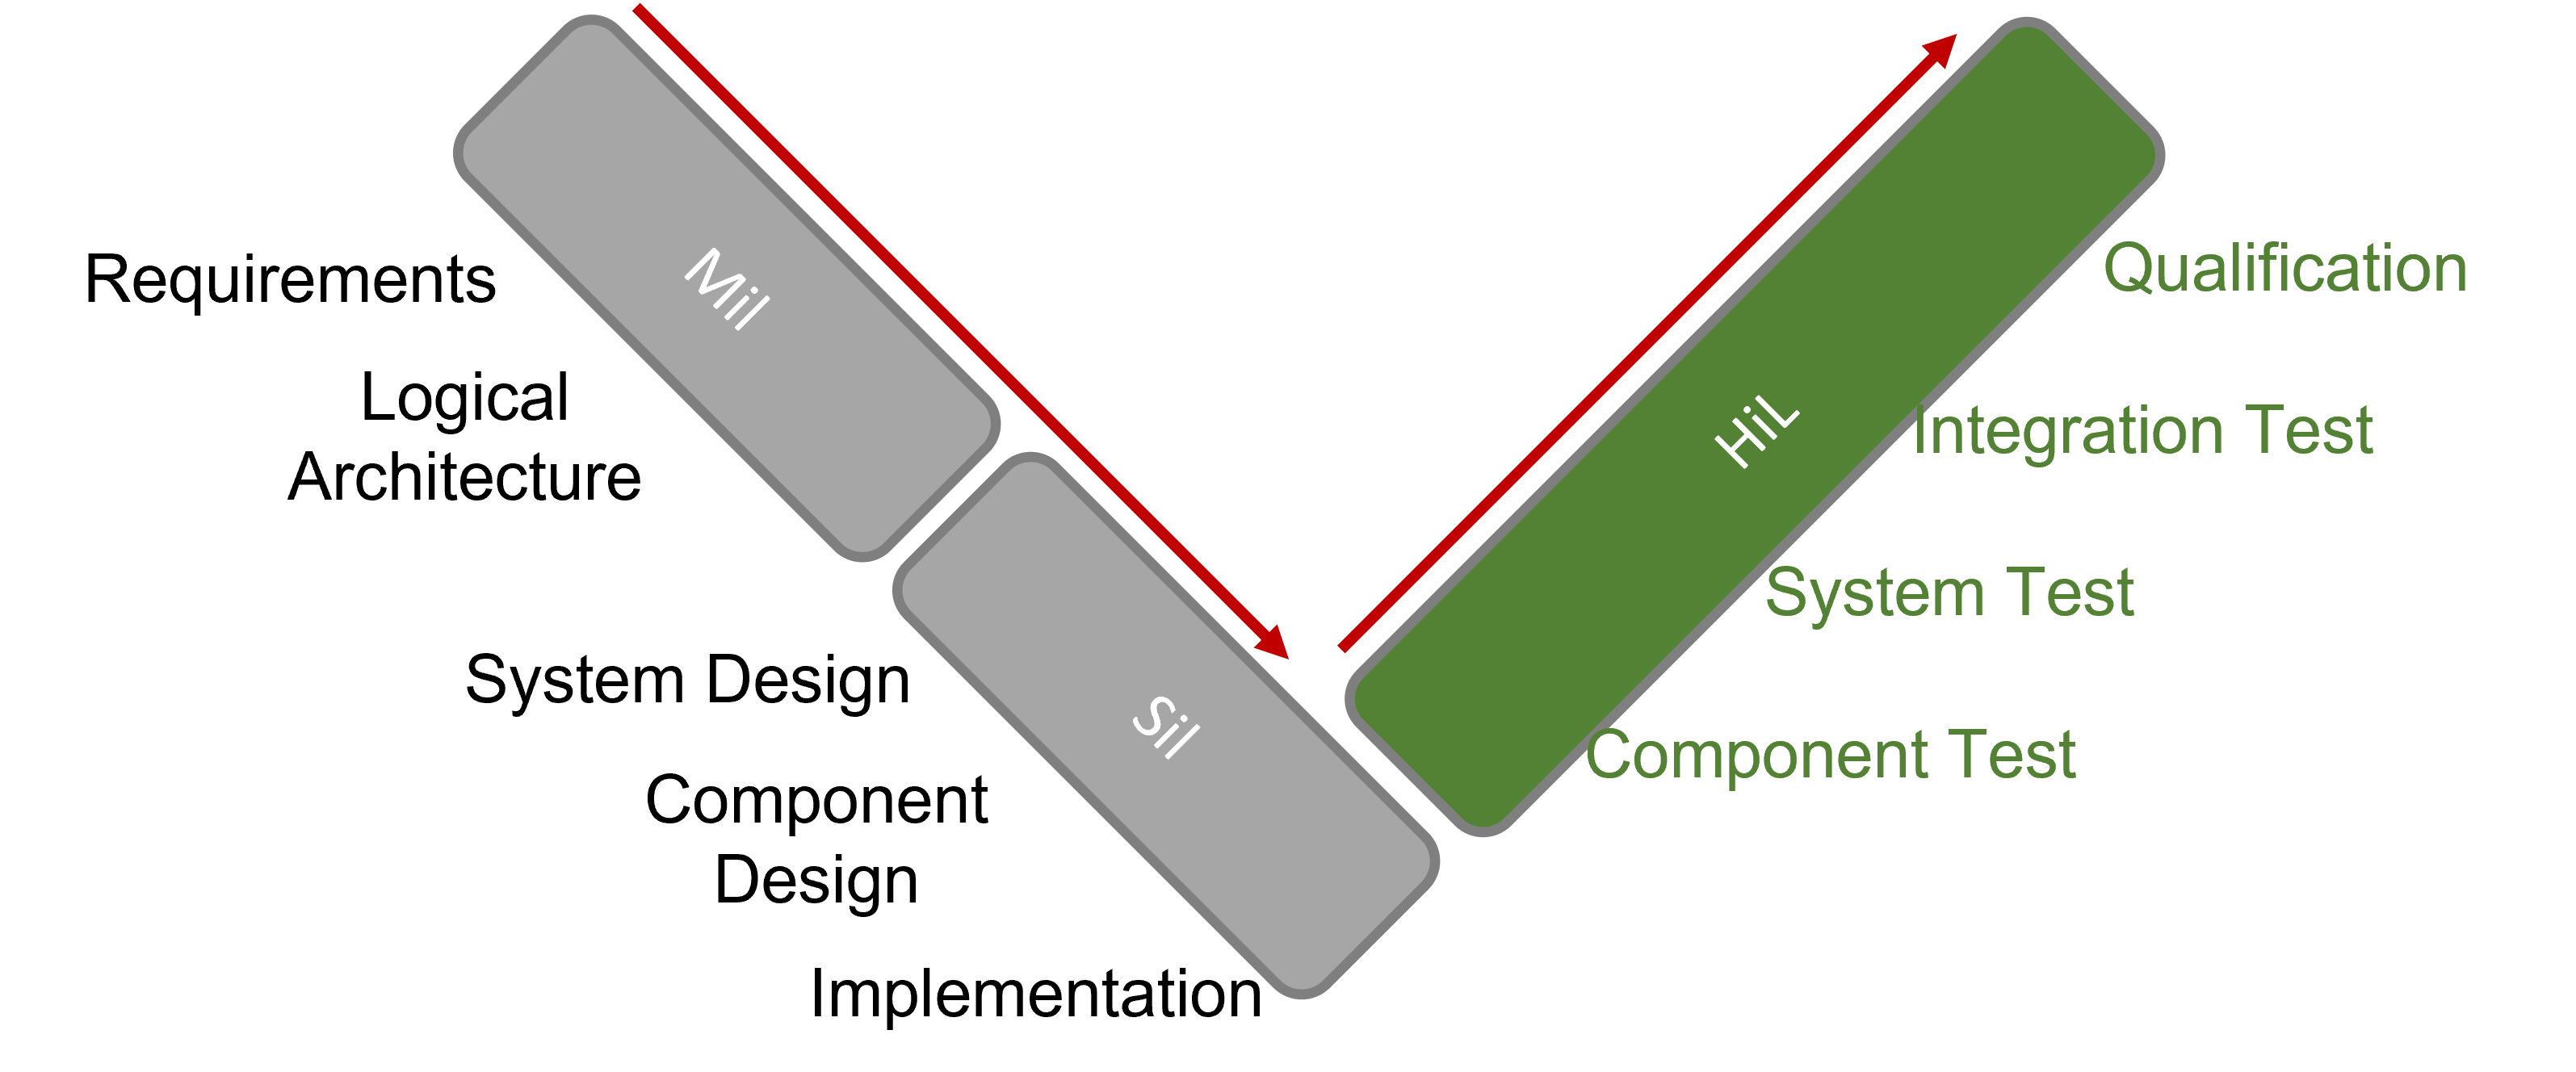
\includegraphics[width=12cm]{Pictures/V Model Component Test.png}
    \caption[V Model Component Test]{V Model Component Test Stage}
    \label{V Model Component Test}
    \end{center}
\end{figure}
\subsection{Component Test}
\subsubsection{Encoder}
\subsubsection{HMI}
\subsubsection{Micro Controller}
\subsubsection{Motor}
\subsubsection{Motor Controller}
\subsubsection{Gearbox}

\subsection{System Test}

\subsection{Integration Test}
\subsubsection{Turning}
\subsubsection{Threading}













